\chapter{Introduction}
\section{General Introduction}

Nowadays, robotics play a very crucial role in industrial area by greatly increasing the industrial productivity. It helps factory workers in many ways:

First, it helps the workers in performing monotonous and tedious task. As humans are bad with dealing the same task over and over again, it will put high stress in workers physical and mental condition. In contrast, a machine or robot can perform the same task in a loop when programmed to do so. And normally it will achieve the same result which is also one advantage compared to workers result.

Second, it can replace human in doing some dangerous tasks. For instance, welding operation is quite dangerous as the activity deals with high temperature. By having the robot to perform the welding, it greatly reduce the risk for the workers to get burned or accident in the process of welding.

Third, robots are very good to deal with precision and accuracy while humans are not. This makes some operation can only be done by the robots and not manually. One example is making the electronics components such as micro chip, small transistors, etc. 

However, these achievements is done because of a highly structured environment such as heavy industry (for example car assembly) where every parameters are known and fixed. In contrast, robotics performance in light industry are still poor. For instances, assembly of small and fragile parts in electronics, food, and other industries. This is because robotics are still bad in dealing with dynamics and unstructured environment where uncertainities are common. 

\begin{figure}[h]
  \begin{subfigure}[t]{0.5\textwidth}
    \centering
    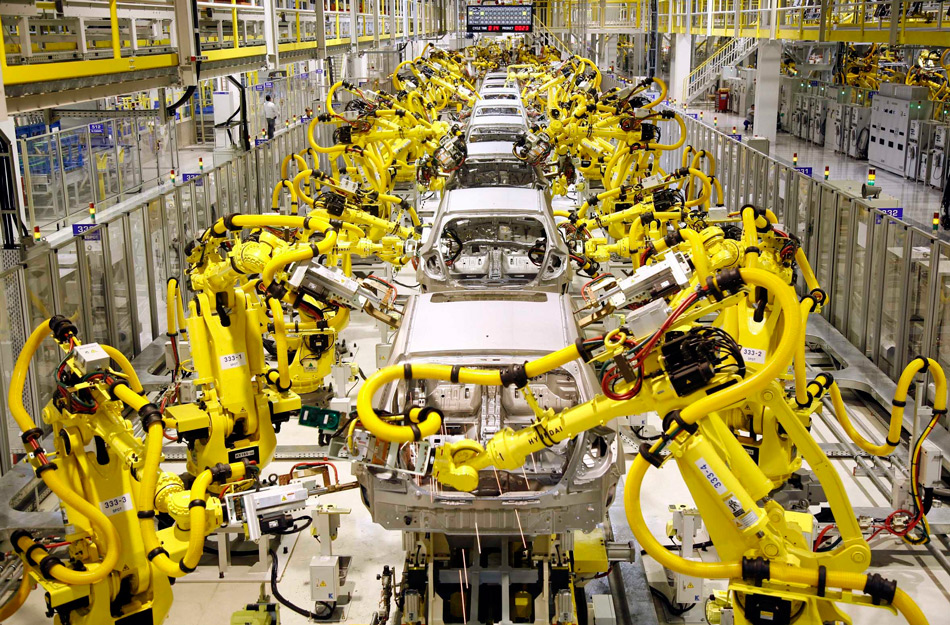
\includegraphics[width = \textwidth ]{heavy_industry} 
    \caption{Robotics in heavy industries}
  \end{subfigure}
  \begin{subfigure}[t]{0.5\textwidth}
    \centering
    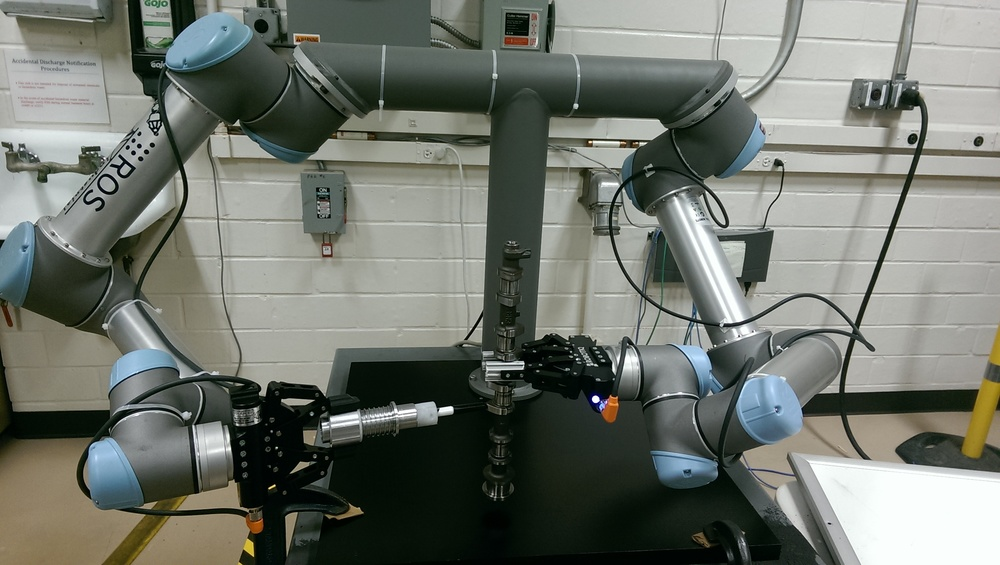
\includegraphics[width = \textwidth ]{assembly_task}
    \caption{Manipulators for assembly task}
  \end{subfigure}
  \caption{Robotics in some applications}
\end{figure}


In light of this, researches and developments in this topic are still intense until now. Many works have attempted to create a framework for fine assembly procedures. Recently, a paper by \cite{aaaa} has introduced the complete framework for fine assembly task. However, there are still always some improvement that can be done.

\section{Objective}


This project aims to estimate the contact force of an assembly robot based on the arm motor currents/torques. Understanding of the mathematical model of the robot’s dynamic, friction, and control theory are considered as important knowledge to work with this project.

The project will be focusing on a certain Denso arm. Thus, the developed systems will be built specifically for this arm. Additionally, some problems that are discussed in this project will be only addressed for this Denso arm and might not be available for other arms.


\section{Scope}


The scope of this project is divided into four parts. First, the project will start from understanding of the general models of robot dynamic and friction. Thus, literature reviews and readings are included in this step. The next step is to perform some experiments to get all necessary data to develop the model. This includes setup preparations, running the experiments, and collections of the data. The third step will be processing all the results and develop the system to estimate the contact force. which after that, validation of the built model to the real data will be the final step.
